\section{Findings}
Figure \ref{fig:boxplot} shows that YOLO consistently is the fastest of the three algorithms across all the sample images. Figure \ref{fig:yolo} shows that YOLO is consistent in its runtime, only one data point is a significant outlier. The outlier might be due to loading the model on the first run. This is also seen on table \ref{tab:statistics} that even though YOLO has a max of 4.441 seconds the interquartile range is just 0.132 seconds and the standard deviation is 0.17 seconds.\\
The data points for the HOG algorithm has the widest range, as seen in table \ref{tab:statistics} it has an interquartile range of 7.823 seconds and a standard deviation of 3.866 seconds. We can see on figure \ref{fig:hog} that there is a gap in the middle with no data points. The gap in the data is due to the difference in the sizes of the images, the smaller the image, the faster it can process the image.\\
Faster R-CNN is consistent in its runtime, as can be seen on figure \ref{fig:rcnn}, it has an interquartile range of 1.023 seconds and a standard deviation of 0.873 seconds, but is still considerably slower than YOLO, almost 6 times slower.

\begin{figure}[!hbt]
\centering
\begin{minipage}{.47\textwidth}
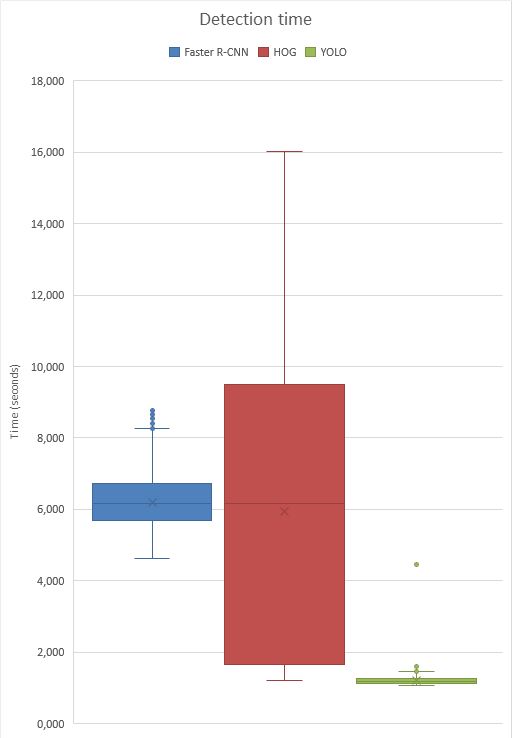
\includegraphics[width=\textwidth]{src/imgs/boxplot.png}
\caption[Boxplot over runtime]{Boxplot over the time it took the three algorithms to finish person detecting. Each of the algorithms has a data size of 600 data points, which has been record from processing 6 different images of varying size and motive.}
\label{fig:boxplot}
\end{minipage}\hspace*{.06\textwidth}%
\begin{minipage}{.47\textwidth}
\centering
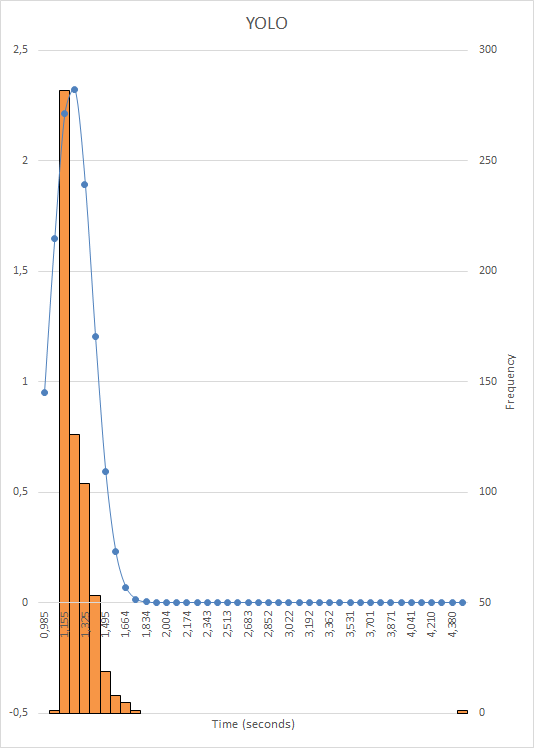
\includegraphics[width=\textwidth]{src/imgs/YOLO_graph.png}
\caption[YOLO Histogram]{Histogram and Bell Curve for the data collected from running YOLO}
\label{fig:yolo}
\end{minipage}
\end{figure}

\begin{table}[!hbt]
\centering
\begin{tabular}{|l|c|c|c|}\hline
&Faster R-CNN&HOG&YOLO\\\hline
Min&4.610&1.196&1.070\\\hline
25-percentile&5.682&1.658&1.130\\\hline
Median&6.166&6.172&1.161\\\hline
75-percentile&6.705&9.481&1.262\\\hline
Max&8.772&16.026&4.441\\\hline
Interquartile Range&1.023&7.823&0.132\\\hline
Mean&6.178&5.929&1.213\\\hline
Standard Deviation.&0.873&3.866&0.170\\\hline
\end{tabular}
\caption[Statistical Variables]{Statistical variables calculated to make boxplot in figure \ref{fig:boxplot}. Time (seconds).}
\label{tab:statistics}
\end{table}

\begin{figure}[!hbt]
\centering
\begin{minipage}{.47\textwidth}
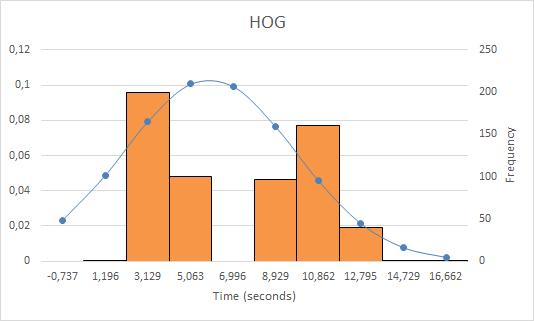
\includegraphics[width=\textwidth]{src/imgs/HOG_graph.png}
\caption[HOG Histogram]{Histogram and Bell Curve for the data collected from running HOG}
\label{fig:hog}
\end{minipage}\hspace*{.06\textwidth}%
\begin{minipage}{.47\textwidth}
\centering
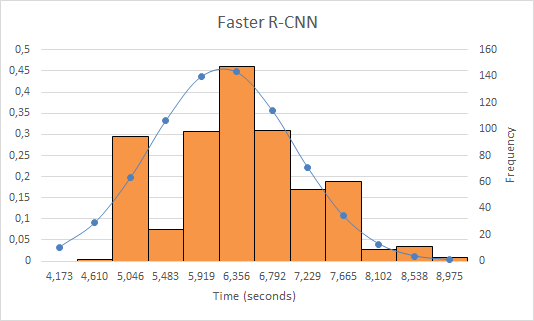
\includegraphics[width=\textwidth]{src/imgs/FasterRCNN_graph.png}
\caption[Faster R-CNN Histogram]{Histogram and Bell Curve for the data collected from running Faster R-CNN}
\label{fig:rcnn}
\end{minipage}
\end{figure}

\noindent The images used for testing contain 13 people. Table \ref{tab:precision} shows that Faster R-CNN found all but also one false positive. YOLO missed one person but it did not get any false positives. HOG got 5 people and detected the legs of one person therefore the .5 point, it also got a false positive.

\begin{table}[!hbt]
\centering
\begin{tabular}{|l|c|c|c|}\hline
&Faster R-CNN&HOG&YOLO\\\hline
Correct Detections&13&5.5&12\\\hline
False Positives&1&1&0\\\hline
\end{tabular}
\caption[Precision Table]{On the 6 images we tested, there were a total of 13 people, this describes how many people the algorithm found out of those with over 90\% confidence.}
\label{tab:precision}
\end{table}
